\documentclass[]{standalone}

\usepackage{adjustbox}

\usepackage{amsmath}
\usepackage{xfrac}
\usepackage{mathrsfs}

\usepackage{circuitikz}
\usepackage{tikz}
\usetikzlibrary{arrows, patterns, decorations.pathmorphing, backgrounds, positioning, fit, petri, shapes, trees, matrix, chains, decorations, decorations.pathreplacing, decorations.fractals, calc,snakes,trees, decorations.markings}

\usepackage{color}
\definecolor{soton}{RGB}{7,51,71}
\colorlet{comms}{red!50!yellow}
\colorlet{payld}{pink!50!purple}
\colorlet{obdh}{green!50!black}

\begin{document}

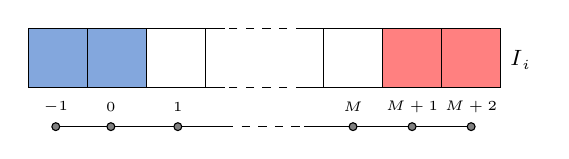
\begin{tikzpicture}

\draw (2.5, 0.75) -- (0, 0.75) -- (0,0) -- (2.5, 0);
\foreach \x in {0.75, 1.5, 2.25}{
    \draw (\x, 0) -- (\x, 0.75);
};

\draw (3.5, 0.75) -- (6, 0.75) -- (6,0) -- (3.5, 0);
\foreach \x in {3.75, 4.5, 5.25}{
    \draw (\x, 0) -- (\x, 0.75);
};

\draw[dashed] (3.5, 0.75) -- (2.5, 0.75);
\draw[dashed] (3.5, 0.) -- (2.5, 0);

\draw[fill=cyan!50!blue!50] (0,0) rectangle (0.75,0.75);
\draw[fill=cyan!50!blue!50] (1.5,0) rectangle (0.75,0.75);
\node at (0.35,-0.25) {\tiny{$-1$}};
\node at (1.05,-0.25) {\tiny{$0$}};
\node at (1.9,-0.25) {\tiny{$1$}};

\draw[fill=red!50] (5.25,0) rectangle (4.5,0.75);
\draw[fill=red!50] (5.25,0) rectangle (6,0.75);
\node at (5.625,-0.25) {\tiny{$M+2$}};
\node at (4.875,-0.25) {\tiny{$M+1$}};
\node at (4.125,-0.25) {\tiny{$M$}};

\draw (0.35, -0.5) -- (2.5, -0.5);
\draw (3.5, -0.5) -- (5.625, -0.5);
\draw[dashed] (2.5, -0.5) -- (3.5, -0.5);
\foreach \x in{0.35, 1.05, 1.9, 5.625, 4.875, 4.125}{
    \draw[fill=black!50] (\x, -0.5) circle (0.05);
    };

\node[right] at (6,0.35) {\footnotesize{$I$}\tiny{$_i$}};

\end{tikzpicture}


\end{document}